\documentclass[presentation.tex]{subfiles}

\begin{document}


\begin{frame}
  \frametitle{Structural Changes in Time Series Models}
  There are three types of changes over time that are of
    interest to the earth science research:
    \begin{enumerate}
    \item \textbf{Seasonal change}: changes that happen within a season (e.g. year)
    \item \textbf{Gradual change}: changes that are caused by interannual climate
      variability.
    \item \textbf{Abrupt change}: rapid changes that are triggered by deforestation,
      floods, fires and similar.
    \end{enumerate}
\end{frame}

\begin{frame}
  \frametitle{BFAST}
  \begin{itemize}
    \item 
      In the paper from 2010, Verbesselt et. al outline a generic change detection approach
      that combines iterative decomposition into trend, seasonal and remainder components and detection
      and characterizing of breakpoints within the trend and seasonal components.
    \item 
      For BFAST, we consider a following data model:
      \[
      Y_t = T_t + S_t + R_t, \quad t = 1,...,n
      \]
      where:
      \begin{itemize}
      \item $Y_t$ is the observation at time $t$
      \item $T_t$ is the trend component at time $t$
      \item $S_t$ is the seasonal component at time $t$
      \item $R_t$ is the remainder component at time $t$
      \item $n$ is the number of observations in time series
      \end{itemize}
  \end{itemize}
\end{frame}

\begin{frame}
\frametitle{BFAST Example - \texttt{harvest}}
\begin{figure}[H]
  \centering
  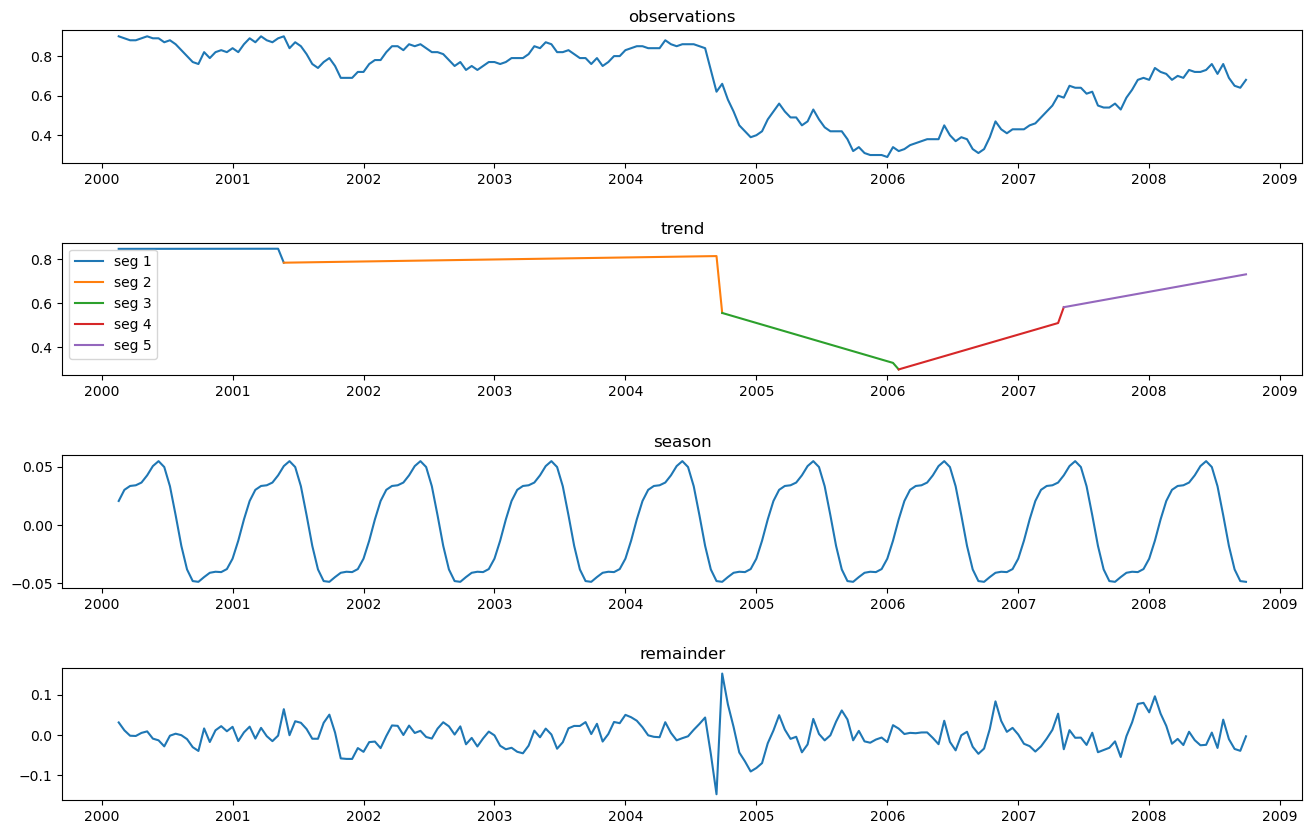
\includegraphics[width=0.9\textwidth]{imgs/harvest.png}
  \caption{Normalized Difference Vegetation Index (NDVI) time series for a pine plantation,
    with 23 observation per year. NDVI is an estimate of the density of green on an area of land.
    There are 4 breakpoints in the trend component. Harmonic seasonal model}
\end{figure}
\end{frame}


\begin{frame}
\frametitle{BFAST Example - \texttt{simts}}
\begin{figure}[H]
  \centering
  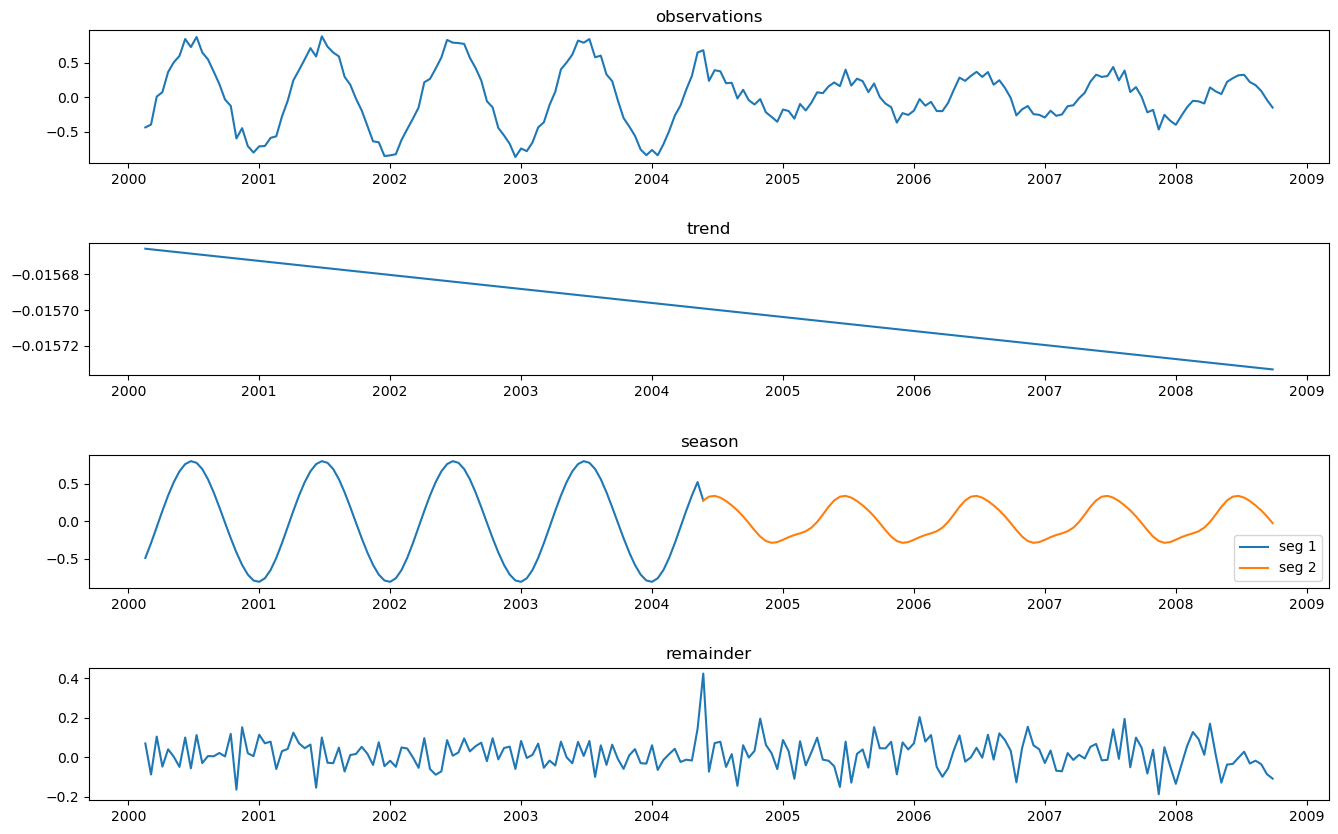
\includegraphics[width=0.9\textwidth]{imgs/simts.png}
  \caption{Simulated seasonal 16-day NDVI time series. The seasonal
    component has a single breakpoint. Harmonic seasonal model}
\end{figure}
\end{frame}

\begin{frame}
\frametitle{BFAST Example - \texttt{nile}}
\begin{figure}[H]
  \centering
  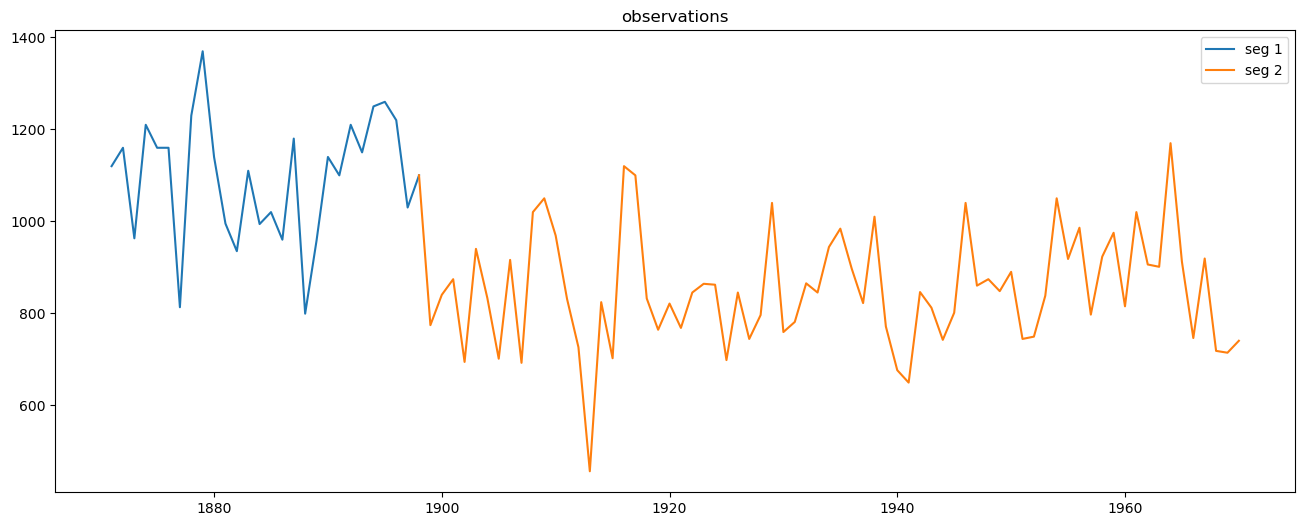
\includegraphics[width=0.9\textwidth]{imgs/nile.png}
  \caption{Measurements of the annual flow of the river Nile with apparent
    breakpoint near 1898 when the dam was built. There is no seasonal
    component, since there is one observation each year}
\end{figure}
\end{frame}


\begin{frame}
\frametitle{BFAST Example - \texttt{ndvi}}
\begin{figure}[H]
  \centering
  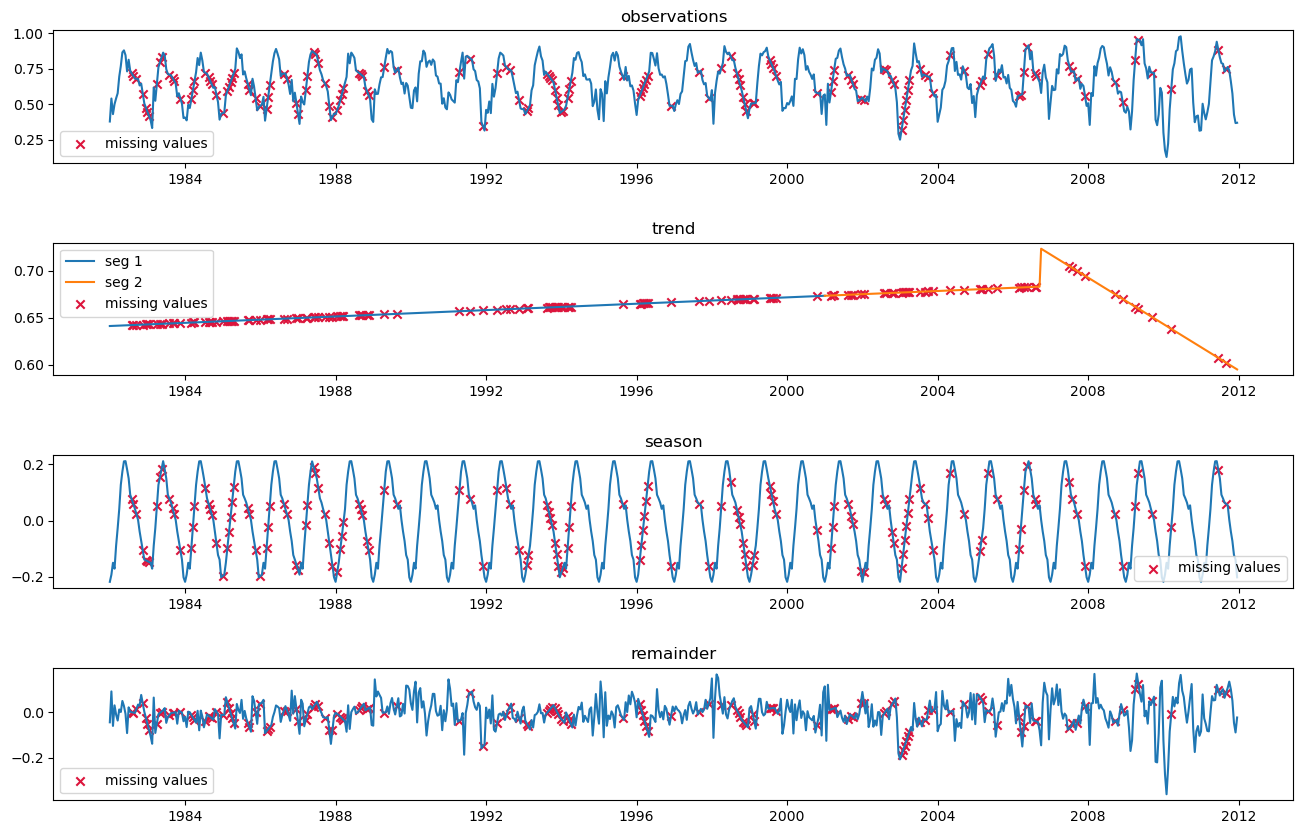
\includegraphics[width=0.9\textwidth]{imgs/ndvi.png}
  \caption{A random NDVI time series with missing values. Frequency is set to 24.
    There is a single breakpoint in the trend component. ``dummy'' seasonal model.}
\end{figure}
\end{frame}

\begin{frame}
  \frametitle{Trend Component}
  \begin{itemize}
  \item 
  We assume that $T_t$ is piecewise linear and has breakpoints $t_1^*,\hdots, t_m^*$,
  where $m$ is the number of breakpoints in the trend component and set $t_0^* = 0$.
  Then, the trend component can be described as
  \[
  T_t = \alpha_j + \beta_j t \quad \text{for}\quad t^*_{j-1}<t\leq t_j^*
  \]
  where:
  \begin{itemize}
  \item $j$ is the number of the next breakpoint, i.e. $j = 1,...,m$.
  \item $\alpha_j$ and $\beta_j$ are the corresponding linear coefficients
  \end{itemize}
  %% \item In matrix form:
  %%   \[
  %%   \mathrm{T} = \mathrm{X} \beta
  %%   \]
  %%   \[
  %%   \mathrm{T} = 
  %%   \begin{bmatrix}
  %%     T_1 \\
  %%     T_2 \\
  %%     \vdots \\
  %%     T_n 
  %%   \end{bmatrix}
  %%   \quad
  %%   \mathrm{X} = 
  %%   \begin{bmatrix}
  %%     1 & T_1 \\
  %%     1 & T_2 \\
  %%     \vdots & \vdots \\
  %%     1 & T_n 
  %%   \end{bmatrix}
  %%   \quad
  %%   \beta =
  %%   \begin{bmatrix}
  %%     \alpha \\
  %%     \beta 
  %%   \end{bmatrix}
  %%   \]
  %% \item 
  %%   One way, in which we can characterize the abrupt changes in the trend component is by
  %%   calculating the magnitude of the change:
  %%   \[
  %%   \operatorname{Magnitude}(j) = T_{j-1} - T_{j} = (\alpha_{j-1} - \alpha_j) + (\beta_{j-1} - \beta_j)t
  %%   \]
  %%   where $j = 1,...,m$.
  \end{itemize}
\end{frame}

\begin{frame}
  \frametitle{Seasonal Component}
  \begin{itemize}
  \item 
    There are two seasonal models that were introduced by Verbesselt et al.:
    Harmonic and ``dummy''. This presentation only covers the former.
    \item 
      The breakpoints in the seasonal component can occur at different times than the
      breaks in the trend component. Let
      $t_1^{\#},\hdots, t_p^{\#}$ be the breakpoints in the seasonal component,
      where $p$ is the number of breakpoints and $t_0^{\#} = 0$.
    \item 
      
      For $t_{j-1}^{\#} < t \leq t_j^{\#}$, the seasonal term can be expressed as:
    \[
    S_t =
    \sum_{k=1}^{K}\left[\gamma_{j, k} \sin \left(\frac{2 \pi k t}{s}\right)+
      \theta_{j, k} \cos \left(\frac{2 \pi k t}{s}\right)\right]
    \]
where
\begin{itemize}
\item $K$ is the harmonic term, i.e. the number of pairs of harmonic terms:
  ($K=3$ is used in BFAST)
\item $\gamma_{j, k}$ and $\theta_{j, k}$ are the seasonal coefficients
\item $t$ is the observation time.
\item $s$ is the period of seasonality (e.g. number of observations per year)
\end{itemize}
  \end{itemize}
\end{frame}

%% \begin{frame}
%%   \frametitle{Seasonal Component - Harmonic Model Continued}
%%   In order to apply the model to the time-series s.t. it could be used by the
%%   breakpoint estimation algorithm, we need to compute the matrix form of the
%%   harmonic model (for $K=3$):
%%   \[
%%   X_{h} =
%%   \begin{bmatrix}
%%     \sin\nicefrac{2 \pi}{f} & \cos\nicefrac{2 \pi}{f} & \sin\nicefrac{4 \pi}{f} & \cos\nicefrac{4
%%       \pi}{f} &  \sin\nicefrac{6 \pi}{f} & \cos\nicefrac{6 \pi}{f} \\
%%     \sin\nicefrac{4 \pi}{f} & \cos\nicefrac{4 \pi}{f} & \sin\nicefrac{8 \pi}{f} & \cos\nicefrac{8
%%       \pi}{f} &  \sin\nicefrac{12 \pi}{f} & \cos\nicefrac{12 \pi}{f} \\
%%     \vdots & \vdots  & \vdots & \vdots & \vdots & \vdots \\
%%     \sin\nicefrac{2 \pi n}{f} & \cos\nicefrac{2 \pi n}{f} & \sin\nicefrac{4 \pi n}{f} &
%%     \cos\nicefrac{4 \pi n}{f} &  \sin\nicefrac{6 \pi n}{f} & \cos\nicefrac{6 \pi n}{f}
%%   \end{bmatrix}
%%   \]
%%   $X_h$ has $n$ rows and $2K$ columns.
%% \[
%% \hat{S} = X_{\text{h}} \omega
%% \]
%% where $\omega$ is a $(1 \times 2K)$ vector
%% $(\gamma_{1, 1}, \; \theta_{1, 1},\;  \gamma_{1, 2},\;  \theta_{1, 2},\; \gamma_{p, 3},\;  \theta_{p, 3})^{\top}$
%% \end{frame}

\begin{frame}
  \frametitle{BFAST Algorithm Steps}
  \begin{itemize}
  \item \textbf{Estimate $S_t$ using STL decomposition, resulting in $\hat{S}_t$}
  \item Iterate, until the number and position of the breakpoints do
    not change during the iteration or the maximum allowed number of iterations
    is reached:
    \begin{enumerate}
    \item \textbf{Calculate the deasonalized time series: $V_t = Y_t - \hat{S}_t$}
    \item \textbf{Apply the OLS-MOSUM test} to $V_t$
      If the returned p-value is lower than the significance level $\alpha$,
      \textbf{estimate the number and position of the trend components} using the
      breakpoint estimation algorithm by Bai and Perron.
    \item \textbf{Compute the trend coefficients} $\alpha_j$ and $\beta_j$ for
      $j = 1, \hdots, m$ using linear regression. Set the trend estimate
      $\hat{T}_t = \hat{\alpha}_j + \hat{\beta}_j t$ for
      $t = t^*_{j-1} + 1, \hdots, t^*_j$.
    \item \textbf{Calculate the detrended time series}: $W_t = Y_t - \hat{T}_t$
    \item \textbf{Apply the OLS-MOSUM test} to $W_t$
    If the test results show that the breakpoints are present in the
      seasonal data, \textbf{estimate the number and position of the
      breakpoints in the seasonal component} using the breakpoint estimation
      algorithm
    \item \textbf{Compute the coefficients for the seasonal component
      and reconstruct $\hat{S}_t$} from the chosen seasonal model and seasonal
      coefficient
  \end{enumerate}
%% \item \textbf{Return} $\hat{T}_t$, $\hat{S}_t$, $(t_1^*, \hdots, t_m^*)$, $(t_1^{\#}, \hdots, t_p^{\#})$
  %% and the maximum breakpoint magnitude.
\end{itemize}

\end{frame}

\end{document}
